% ============================================================
%  SE2RoadNet — Test Prioritization for Self-Driving Cars
%  Restructured to mirror the CGAR/MEMRES deck template:
%   1. Bối cảnh & Phát biểu bài toán
%   2. Công trình liên quan & Khoảng trống nghiên cứu
%   3. RoadFury: Phương pháp nền tảng        (≈ MEMRES)
%   4. SE2RoadNet: Đề xuất của nhóm          (≈ CGAR)
%   5. Đánh giá thực nghiệm
%   6. Hạn chế & Hướng phát triển
%  All figures are CODE-GENERATED (TikZ / matplotlib), no AI images.
%  Compile: pdflatex se2_slides.tex  (twice for TOC/refs)
% ============================================================
\documentclass[aspectratio=169,10pt]{beamer}

\usetheme{metropolis}
\usecolortheme{metropolis}
\usefonttheme{professionalfonts}
\setbeamertemplate{frame numbering}[fraction]
\setbeamertemplate{itemize item}{\textcolor{mLightBrown}{\tiny$\blacktriangleright$}}
\setbeamertemplate{itemize subitem}{\textcolor{mLightBrown!70}{\tiny$\bullet$}}
% Clean presentation captions: no "Figure N:" label, grey italic
\setbeamertemplate{caption}{\centering\footnotesize\itshape\color{gray}\insertcaption\par}
\setbeamerfont{caption}{size=\footnotesize}

% -- Packages --
\usepackage{amsmath, amssymb}
\usepackage[utf8]{inputenc}
\usepackage{vietnam}
\usepackage[english]{babel}
\usepackage{booktabs}
\usepackage{multirow}
\usepackage[table]{xcolor}
\usepackage{graphicx}
\usepackage{adjustbox}
\usepackage{hyperref}
\usepackage{parskip}
\usepackage{tikz}
\usepackage{pgfplots}
\pgfplotsset{compat=1.18}
\usetikzlibrary{arrows.meta, positioning, fit, backgrounds, decorations.pathreplacing,
                shapes.geometric, calc, decorations.pathmorphing}
\usepackage{mdframed}
\usepackage{pifont}
\newcommand{\cmark}{\ding{51}}
\newcommand{\xmark}{\ding{55}}

% ============================================================
%  PALETTE (matches the template deck)
% ============================================================
\definecolor{mDarkTeal}{HTML}{23373B}
\definecolor{mLightBrown}{HTML}{EB811B}
\definecolor{softgray}{HTML}{F2F4F7}
\definecolor{tealtint}{HTML}{D6DEE0}

\colorlet{navydeep}{mDarkTeal}
\colorlet{navymid}{mDarkTeal!75}
\colorlet{accent}{mLightBrown}
\colorlet{success}{green!50!black}
\colorlet{alert}{red!70!black}
\colorlet{lightnavy}{tealtint}

\hypersetup{colorlinks=true, urlcolor=mLightBrown, linkcolor=mDarkTeal}
\renewcommand{\arraystretch}{1.15}

% --- Semantic colored boxes (two blind-spots + fix) ---
\definecolor{cRot}{HTML}{B85450}      % terracotta — rotation sensitivity
\definecolor{cRes}{HTML}{C8A951}      % gold — resolution sensitivity
\definecolor{cInv}{HTML}{2C3E6B}      % navy — invariance
\definecolor{cRotL}{HTML}{F2E6E5}
\definecolor{cResL}{HTML}{F5F0E0}
\definecolor{cInvL}{HTML}{EEF0F5}

\newmdenv[topline=false,bottomline=false,rightline=false,
  linewidth=2.5pt,linecolor=cRot,
  innerleftmargin=6pt,innerrightmargin=4pt,
  innertopmargin=3pt,innerbottommargin=3pt,
  backgroundcolor=cRotL]{rotbox}
\newmdenv[topline=false,bottomline=false,rightline=false,
  linewidth=2.5pt,linecolor=cRes,
  innerleftmargin=6pt,innerrightmargin=4pt,
  innertopmargin=3pt,innerbottommargin=3pt,
  backgroundcolor=cResL]{resbox}

\newcommand{\takeaway}[1]{%
  \vspace{0.3em}%
  \begin{mdframed}[linecolor=mLightBrown,linewidth=1.2pt,
    backgroundcolor=mLightBrown!8,
    innertopmargin=4pt,innerbottommargin=4pt,
    innerleftmargin=8pt,innerrightmargin=8pt,roundcorner=2pt]
  \centering\footnotesize\bfseries\color{mDarkTeal} #1
  \end{mdframed}}

% Path helpers
\graphicspath{{./figures/}{../paper/present/}}

% ============================================================
%  TITLE METADATA
% ============================================================
\title{Test Prioritization for Self-Driving Cars}
\subtitle{SE2RoadNet — Bất biến SE(2) bằng kiến trúc}
\author{Trần Chí Nguyên, Huỳnh Trung Kiệt, Đào Sỹ Duy Minh}
\institute{University of Science, VNU-HCM}
\date{ICST 2026}

\begin{document}

% ==================== TITLE ====================
{
\setbeamertemplate{footline}{}
\begin{frame}
\vspace{0.4em}
\begin{columns}[c]
\column{0.18\textwidth}
\centering

\includegraphics[height=2.0cm]{hcmus.png}

\column{0.64\textwidth}
\centering
\large\textbf{The Self-Driving Car Testing Competition}\\[0.3em]
\footnotesize organized jointly with the International Conference on\\
Software Testing, Verification and Validation \textbf{(ICST)}\\[0.7em]
\large\textcolor{navydeep}{\textbf{Test Prioritization for Self-Driving Cars}}\\[0.2em]
\normalsize\textbf{SE2RoadNet} — \footnotesize\textit{bất biến SE(2) bằng kiến trúc}

\column{0.18\textwidth}
\centering

\includegraphics[height=1.6cm]{icst_logo.jpg}
\end{columns}

\vspace{1.4em}
\begin{columns}[c]
\column{0.46\textwidth}
\begin{block}{Tóm tắt đề tài}
\scriptsize
Xếp hạng kịch bản kiểm thử SDC để \textbf{lộ lỗi sớm}; mô hình \textbf{bất biến phép xoay / lấy mẫu} bằng \emph{ràng buộc kiến trúc}, không bằng augmentation.
\end{block}

\column{0.40\textwidth}
\begin{block}{Thành viên nhóm}
\scriptsize
\begin{itemize}
  \item Trần Chí Nguyên -- 23102244
  \item Huỳnh Trung Kiệt -- 23122039
  \item Đào Sỹ Duy Minh -- 23122041
\end{itemize}
\end{block}
\end{columns}

\vspace{1.0em}
\centering
\scriptsize University of Science, VNU-HCM \quad$\cdot$\quad ICST 2026
\end{frame}
}

% ==================== OUTLINE ====================
\begin{frame}{Nội dung chính}
\begin{enumerate}
  \item Bối cảnh \& Phát biểu bài toán
  \item Công trình liên quan \& Khoảng trống nghiên cứu
  \item RoadFury: Phương pháp nền tảng
  \item \textbf{\color{mLightBrown}SE2RoadNet: Đề xuất của nhóm}
  \item Đánh giá thực nghiệm
  \item Hạn chế \& Hướng phát triển
\end{enumerate}

\vspace{0.8em}
\centering\scriptsize\color{gray}
\textit{($+$ Backup slides cho Q\&A: APFD worked-example, Multi-trial, AUC vs APFD, Resolution probe, Chi phí ở quy mô lớn)}
\end{frame}

% ============================================================
\section{Bối cảnh \& Phát biểu bài toán}
% ============================================================

% --- Context / big picture (all-TikZ infographic) ---
\begin{frame}{Bối cảnh: Kiểm thử Self-Driving Car trong mô phỏng}
\centering
\begin{tikzpicture}[font=\scriptsize,
  cardbase/.style={rounded corners=5pt, line width=1pt,
               text width=3.5cm, align=left, inner sep=7pt, minimum height=2.1cm, anchor=north},
  cardN/.style={cardbase, draw=navydeep, fill=navydeep!7},
  cardO/.style={cardbase, draw=mLightBrown, fill=mLightBrown!7},
  cardG/.style={cardbase, draw=success, fill=success!7},
  arr/.style={-{Stealth[length=2.5mm]}, line width=1.3pt, mDarkTeal!75},
]
  % left: many scenarios
  \node[cardN] (sc) at (-5.1,2.6) {%
    \textbf{\normalsize\color{navydeep}Hàng ngàn kịch bản}\\[3pt]
    Sinh tự động các con đường (ambiegen, frenetic\dots) trên \textbf{BeamNG.tech}.
    Mỗi đường $=$ một bài kiểm thử giữ làn.};
  % middle: simulation cost
  \node[cardO] (sim) at (0,2.6) {%
    \textbf{\normalsize\color{mLightBrown!85!black}Mô phỏng tốn kém}\\[3pt]
    Mỗi kịch bản chạy vật lý thời gian thực $\Rightarrow$ \textbf{nhiều giờ CPU} cho toàn tập.};
  % right: prioritize
  \node[cardG] (pri) at (5.1,2.6) {%
    \textbf{\normalsize\color{success!55!black}Phải ưu tiên}\\[3pt]
    Xếp thứ tự để \textbf{lỗi lộ sớm} $\Rightarrow$ chạy ít kịch bản đầu là đủ, cắt 50--80\% thời gian.};
  \draw[arr] (sc.east) -- (sim.west);
  \draw[arr] (sim.east) -- (pri.west);

  % bottom: a stylised winding road with PASS/FAIL markers (pure TikZ)
  \begin{scope}[shift={(0,-1.15)}]
    \draw[line width=8pt, mDarkTeal!18, line cap=round]
      plot[smooth, domain=-5.2:5.2, samples=80] ({\x}, {0.30*sin(deg(1.05*\x))+0.10*sin(deg(2.4*\x))});
    \draw[line width=1.2pt, white, dashed, dash pattern=on 5pt off 5pt]
      plot[smooth, domain=-5.2:5.2, samples=80] ({\x}, {0.30*sin(deg(1.05*\x))+0.10*sin(deg(2.4*\x))});
    \node[success, font=\bfseries\scriptsize] at (-3.6,0.62) {\cmark\ PASS};
    \node[alert,   font=\bfseries\scriptsize] at (2.4,-0.62) {\xmark\ FAIL};
    \fill[mLightBrown] (-1.0,{0.30*sin(deg(-1.05))+0.10*sin(deg(-2.4))}) circle (2.4pt);
  \end{scope}
\end{tikzpicture}

\takeaway{Một thay đổi nhỏ có thể khiến xe lệch làn ở kịch bản hiếm $\Rightarrow$ cần kiểm thử quy mô lớn, nhưng chạy hết thì quá đắt.}
\end{frame}

% --- Formal problem statement (INPUT -> SCORER -> OUTPUT) ---
\begin{frame}{Phát biểu bài toán \& Tiêu chí đánh giá}
\centering
\begin{tikzpicture}[
  every node/.style={font=\scriptsize},
  iobox/.style={draw=navydeep, fill=navydeep!6, rounded corners=4pt,
                minimum width=3.5cm, minimum height=1.95cm, align=left,
                inner sep=5pt, font=\tiny},
  sys/.style={draw=mLightBrown, fill=mLightBrown!12, rounded corners=4pt,
              minimum width=3.0cm, minimum height=1.95cm, align=center,
              line width=1pt, font=\scriptsize\bfseries},
  outbox/.style={draw=success, fill=success!10, rounded corners=4pt,
                 minimum width=3.5cm, minimum height=1.95cm, align=left,
                 inner sep=5pt, font=\tiny},
  arr/.style={->, very thick, mDarkTeal},
  ok/.style={draw=success, fill=success!15, rounded corners=3pt,
             minimum width=9.7cm, minimum height=0.55cm, align=center,
             font=\scriptsize, line width=0.8pt},
]
  \node[iobox] (in) at (-5.1, 1.6)
    {\textbf{\normalsize\color{navydeep}INPUT}\\[3pt]
     $\bullet$ Đường $=$ chuỗi điểm 2D\\
     \phantom{$\bullet$ }$\mathcal{R}=\{p_1,\dots,p_N\}\subset\mathbb{R}^2$\\
     $\bullet$ $N$ thay đổi: \textbf{64--197} điểm\\
     $\bullet$ Chỉ \textbf{hình học}, không có\\\phantom{$\bullet$ }hành vi xe};

  \node[sys] (sys) at (0, 1.6)
    {\color{mLightBrown}SCORER $f_\theta$\\[2pt]
     \scriptsize\mdseries $\mathcal{R}\!\mapsto\![0,1]$\\ (xác suất FAIL)};

  \node[outbox] (out) at (5.1, 1.6)
    {\textbf{\normalsize\color{success!50!black}OUTPUT}\\[3pt]
     $\bullet$ Hoán vị $\pi$ của $n$ kịch bản\\
     $\bullet$ Sắp \textbf{giảm dần} theo điểm\\
     $\bullet$ Mục tiêu:\\\phantom{$\bullet$ }$\pi^*=\arg\max_\pi \mathrm{APFD}(\pi)$};

  \draw[arr] (in.east) -- (sys.west);
  \draw[arr] (sys.east) -- (out.west);

  \node[ok] (ok) at (0, 0.0)
    {\color{success!50!black}\textbf{Success Criterion:}\;
     lỗi (FAIL) được xếp \emph{càng sớm càng tốt} $\Rightarrow$ APFD cao $\Rightarrow$ tiết kiệm chi phí mô phỏng};
  \draw[arr, success!60!black] (sys.south) -- (ok.north);
\end{tikzpicture}

\vspace{0.4em}
\begin{columns}[T,onlytextwidth]
\column{0.34\textwidth}
\scriptsize
\textbf{\color{navydeep}Cho trước}
\begin{itemize}\setlength{\itemsep}{0pt}\scriptsize
  \item Nhãn train $y\!\in\!\{0,1\}$ (PASS/FAIL)
  \item Cùng \textbf{ngân sách} cho mọi tool
\end{itemize}

\column{0.34\textwidth}
\scriptsize
\textbf{\color{alert}Khó khăn}
\begin{itemize}\setlength{\itemsep}{0pt}\scriptsize
  \item Chỉ có hình học đường, không có phản ứng xe
  \item Tập thi \textbf{out-of-distribution}
\end{itemize}

\column{0.30\textwidth}
\scriptsize
\textbf{\color{mLightBrown}Metric}
\begin{itemize}\setlength{\itemsep}{0pt}\scriptsize
  \item \textbf{APFD} (primary)
  \item AUC (phụ), Rotation $\Delta$
\end{itemize}
\end{columns}
\end{frame}

% --- Why prioritize: cost (APFD curve) ---
\begin{frame}{Vì sao cần ưu tiên kiểm thử?}
\begin{columns}[c]
\column{0.55\textwidth}
\centering
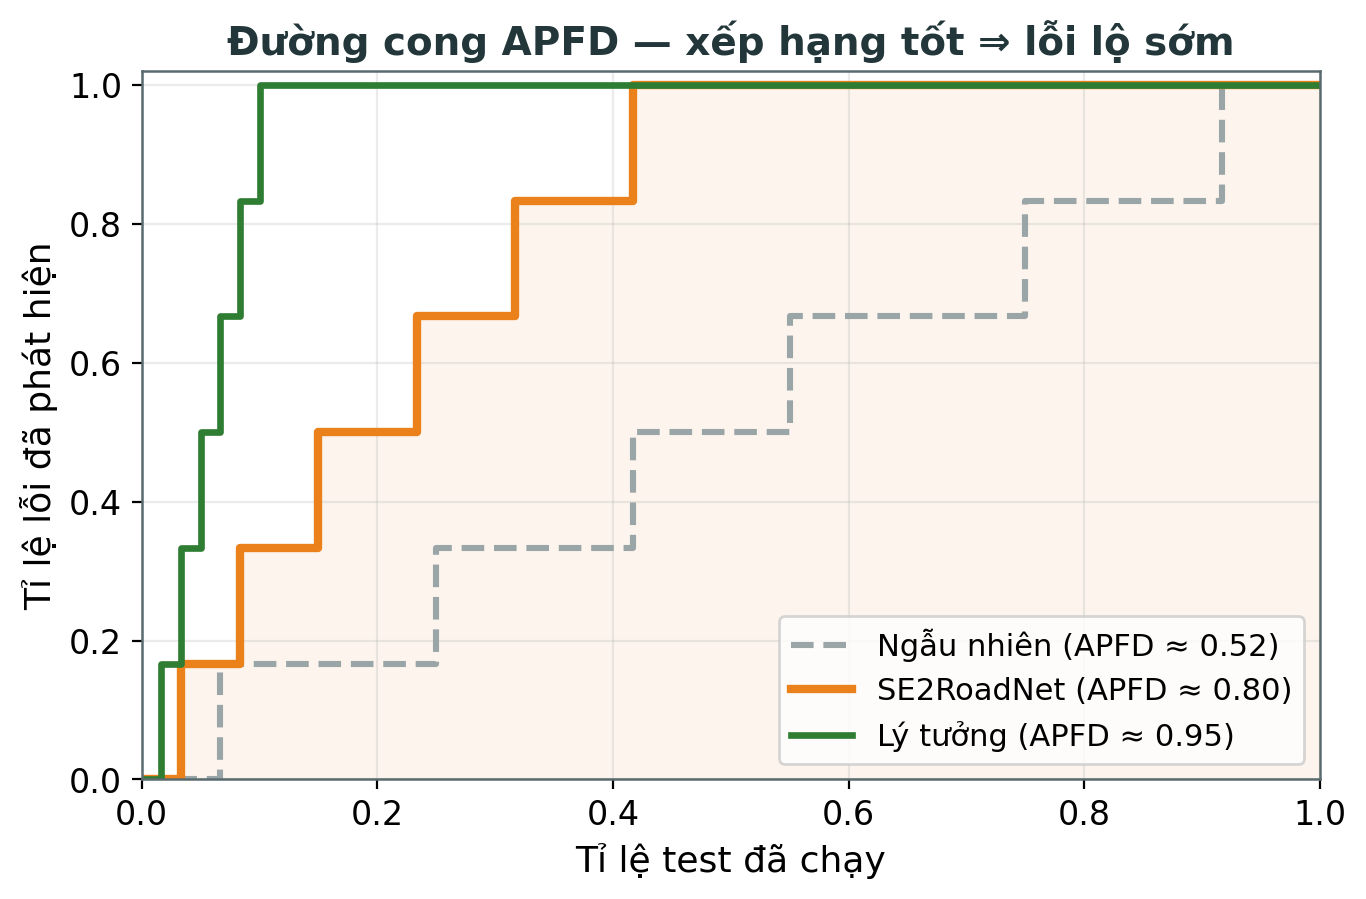
\includegraphics[width=\linewidth]{gen_apfd_curve.png}

\column{0.43\textwidth}
\footnotesize
\textbf{\color{navydeep}Trực giác:}
\begin{itemize}\setlength{\itemsep}{3pt}\scriptsize
  \item Xếp hạng \textcolor{success!55!black}{\textbf{tốt}} $\Rightarrow$ lỗi dồn lên đầu $\Rightarrow$ đường cong dốc đứng từ sớm.
  \item Xếp hạng \textcolor{alert}{\textbf{kém}} $\Rightarrow$ lỗi nằm cuối hàng đợi $\Rightarrow$ tốn nhiều giờ mô phỏng.
  \item \textbf{APFD} đo chính diện tích dưới đường cong này.
\end{itemize}
\vspace{0.3em}
\begin{center}
\fcolorbox{alert}{alert!8}{\parbox{0.95\linewidth}{\centering\scriptsize
  956 kịch bản $\times$ mô phỏng vật lý\\
  $\Rightarrow$ \textbf{\color{alert}nhiều giờ CPU} nếu chạy hết}}
\end{center}
\end{columns}

\takeaway{Ranking tốt cắt 50--80\% chi phí testing — bài toán không phải ``chạy nhanh hơn'' mà là ``chạy đúng thứ tự''.}
\end{frame}

% --- Dataset: SensoDat ---
\begin{frame}{Dataset: SensoDat \small(Birchler et al., MSR 2024)}
\begin{columns}[T]
\column{0.46\textwidth}
\begin{block}{Tổng quan}
\scriptsize
Bộ dữ liệu công khai các kịch bản SDC sinh tự động trên BeamNG.tech, chia 3 split:
\begin{itemize}\setlength{\itemsep}{1pt}
  \item \textbf{Train} -- huấn luyện mô hình.
  \item \textbf{Test (SensoDat)} -- đánh giá in-distribution.
  \item \textbf{Competition} -- 956 kịch bản \textcolor{alert}{\textbf{out-of-distribution}}.
\end{itemize}
\end{block}
\centering\scriptsize
\setlength{\tabcolsep}{4pt}
\begin{tabular}{l r r r}
\toprule
\textbf{Split} & \textbf{N} & \textbf{\%FAIL} & \textbf{Dài (m)} \\
\midrule
Train             & 28\,804 & 38.4\% & 61--454 \\
Test (SensoDat)   &  7\,202 & 38.4\% & 76--433 \\
Competition (OOD) &     956 & \alert{36.9\%} & 129--229 \\
\bottomrule
\end{tabular}

\column{0.52\textwidth}
\centering
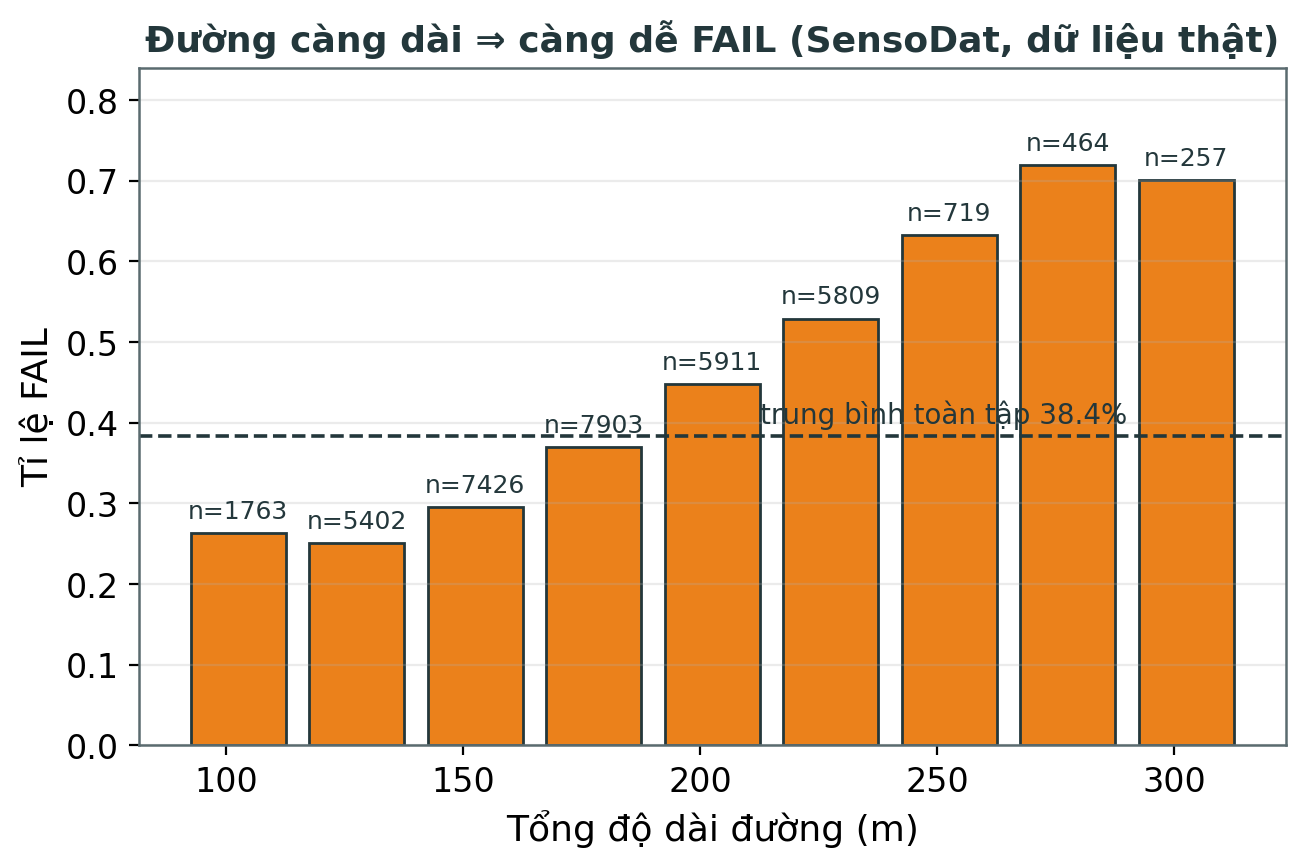
\includegraphics[width=\linewidth]{gen_failrate_by_length.png}\\[0.2em]
\scriptsize\textit{Competition có khoảng độ dài \emph{hẹp hơn} (129--229m) $\Rightarrow$ dịch phân phối (distribution shift).}
\end{columns}
\end{frame}

% --- Sample roads + real screenshot: shape decides label ---
\begin{frame}{Ví dụ kịch bản: hình dạng quyết định nhãn}
\begin{columns}[c]
\column{0.50\textwidth}
\centering
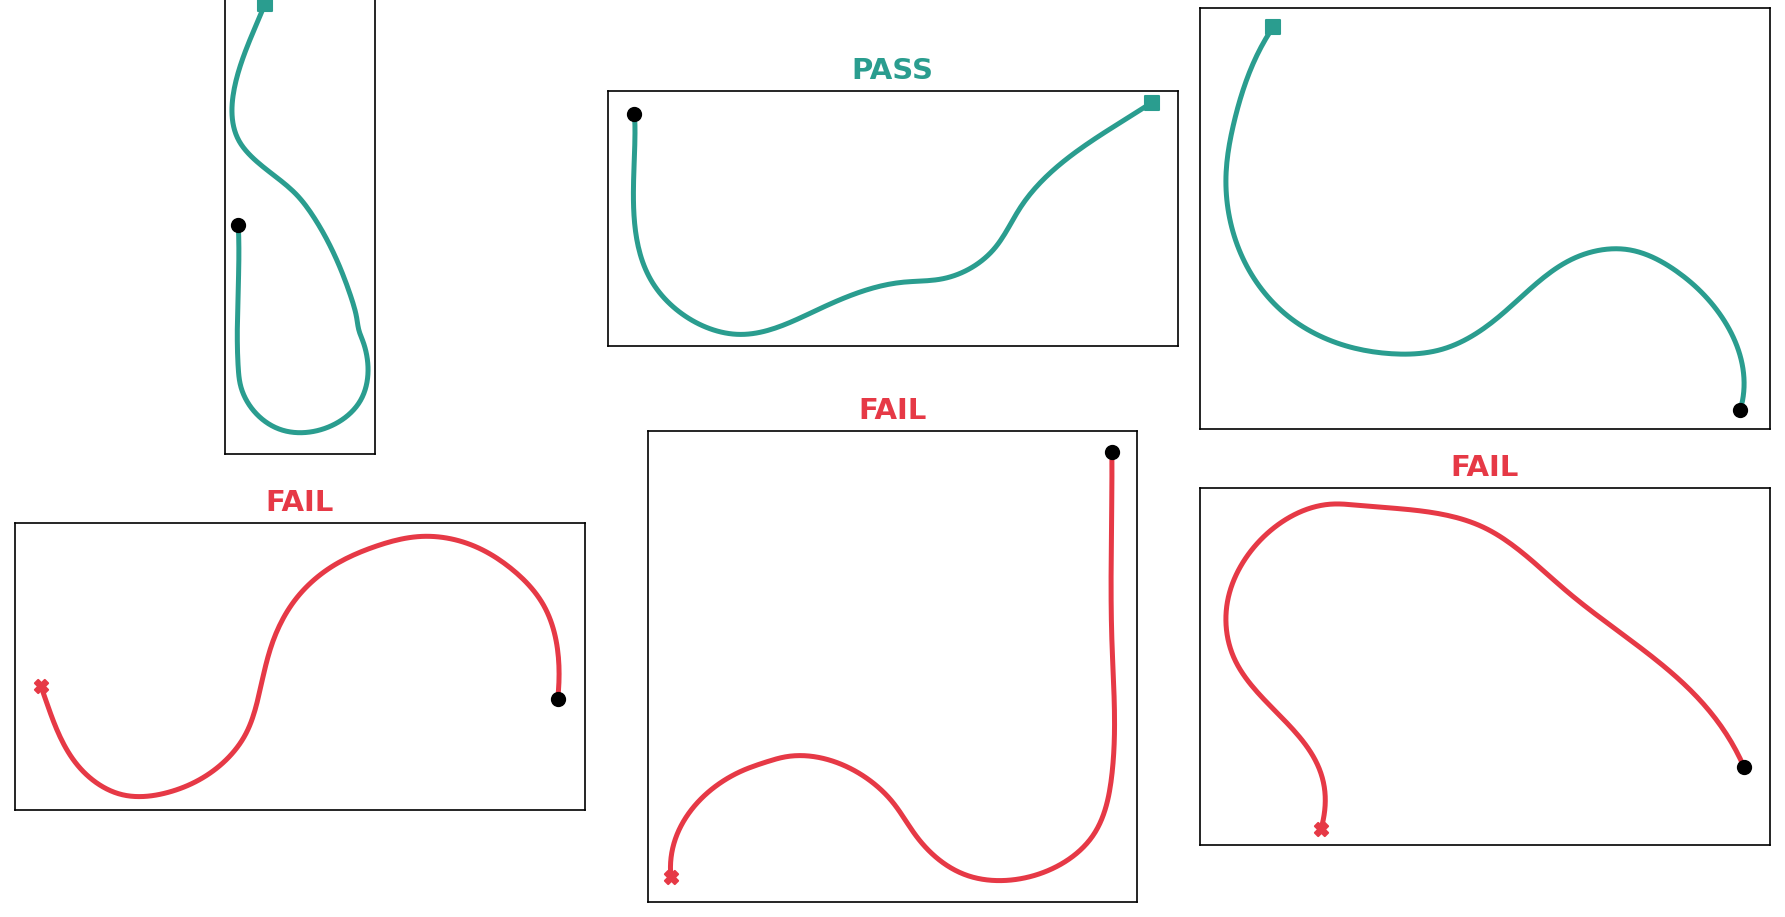
\includegraphics[height=3.55cm]{real_roads_grid.png}\\[0.15em]
{\scriptsize\textit{Đường thật từ SensoDat test split} \;$\cdot$\; \textcolor{success!55!black}{\textbf{PASS}} mượt, \textcolor{alert}{\textbf{FAIL}} chicane gắt}

\column{0.48\textwidth}
\centering
\includegraphics[height=2.05cm]{example.png}\\[0.12em]
{\scriptsize\textit{BeamNG.tech: trái PASS (trong làn) $\cdot$ phải FAIL (lệch làn)}}\\[0.35em]
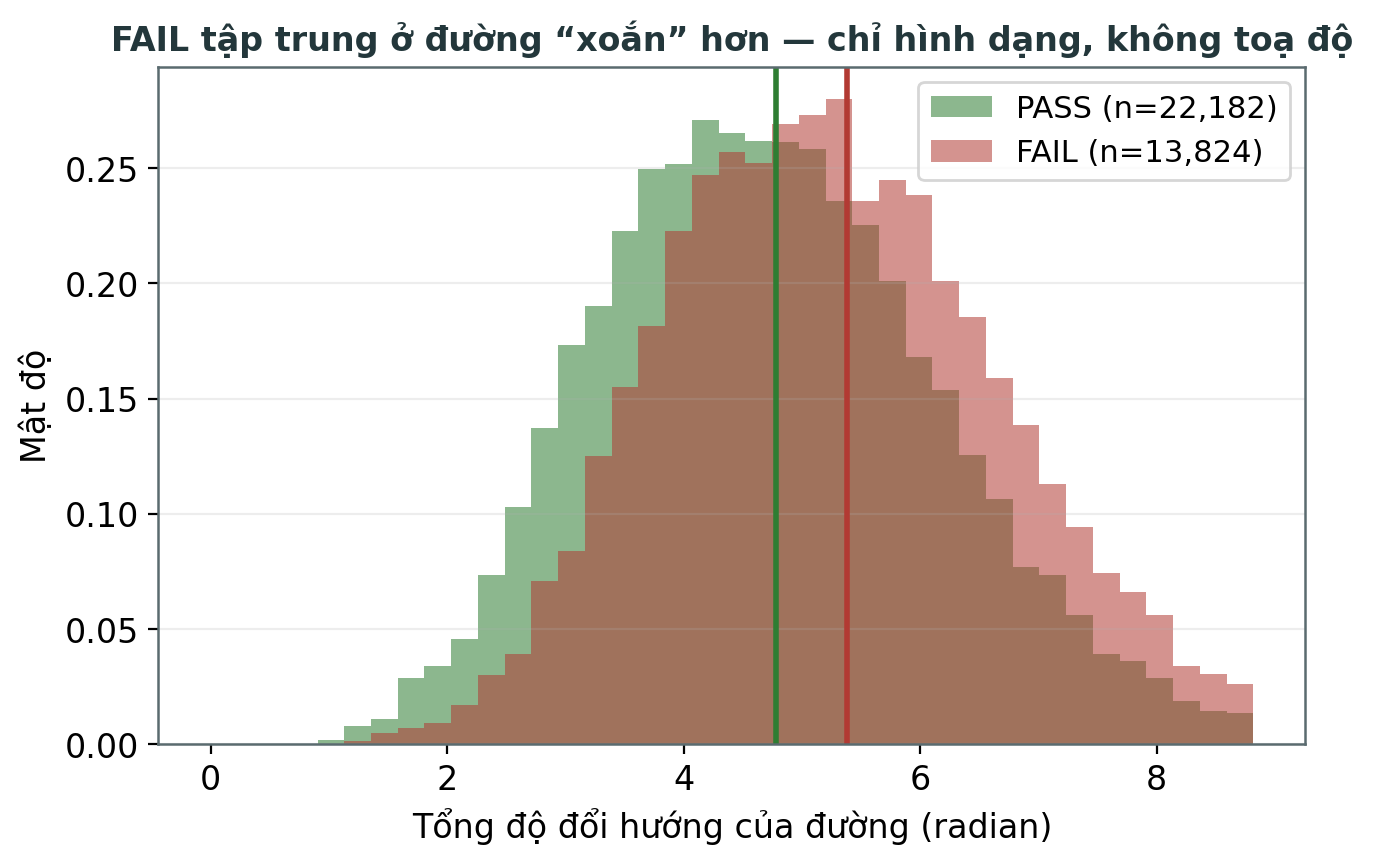
\includegraphics[height=2.85cm]{gen_curvature_signature.png}
\end{columns}

\vspace{0.25em}
\centering\footnotesize\color{mDarkTeal}
$\Rightarrow$ Không có toạ độ $(x,y)$ tuyệt đối nào quyết định nhãn — chỉ \textbf{hình dạng}. Gợi ý cho ràng buộc \textbf{bất biến}.
\end{frame}

% ============================================================
\section{Công trình liên quan \& Khoảng trống nghiên cứu}
% ============================================================

% --- RW 1/2: three approaches ---
\begin{frame}{Related Work: 3 hướng tiếp cận}
\centering
\begin{tikzpicture}[font=\scriptsize,
  rwcard/.style={rounded corners=6pt, line width=1pt, text width=3.5cm,
                 inner sep=9pt, align=left, anchor=north, minimum height=5.3cm},
  rwnum/.style={circle, text=white, font=\bfseries\footnotesize, inner sep=2.6pt},
]
  % 1. Search-based / diversity
  \node[rwcard, draw=navydeep!45, fill=navydeep!4] (c1) at (-3.85,3.0) {%
    \hspace*{0.62cm}\textbf{\normalsize\color{navydeep}Search-based / Diversity}\\[3pt]
    \textcolor{navydeep!25}{\rule{\linewidth}{0.5pt}}\\[4pt]
    \textbf{Ý tưởng:} GA / heuristic chọn tập test \emph{đa dạng} hành vi (SO-SDC-Prioritizer, Greedy-diversity).\\[5pt]
    {\color{success!50!black}\cmark\ \textbf{Ưu:}} không cần nhãn, truyền thống SBST.\\[5pt]
    {\color{alert}\xmark\ \textbf{Hạn chế:}} đa dạng $\neq$ lộ lỗi; đặc trưng phụ thuộc khung.};
  \node[rwnum, fill=navydeep] at (-5.35,2.55) {1};
  % 2. Hand-crafted ML
  \node[rwcard, draw=mLightBrown!55, fill=mLightBrown!6] (c2) at (0,3.0) {%
    \hspace*{0.62cm}\textbf{\normalsize\color{mLightBrown!85!black}Feature-based ML}\\[3pt]
    \textcolor{mLightBrown!30}{\rule{\linewidth}{0.5pt}}\\[4pt]
    \textbf{Ý tưởng:} vài đặc trưng tay $\to$ classifier nhỏ $\to$ rank (ITEP4SDC: MLP 3 đặc trưng).\\[5pt]
    {\color{success!50!black}\cmark\ \textbf{Ưu:}} rẻ, dễ giải thích.\\[5pt]
    {\color{alert}\xmark\ \textbf{Hạn chế:}} ít đặc trưng, phụ thuộc khung, tinh chỉnh theo từng bench.};
  \node[rwnum, fill=mLightBrown!85!black] at (-1.5,2.55) {2};
  % 3. Deep / visual
  \node[rwcard, draw=success!55!black!45, fill=success!55!black!5] (c3) at (3.85,3.0) {%
    \hspace*{0.62cm}\textbf{\normalsize\color{success!45!black}Deep: GNN / CNN / Transformer}\\[3pt]
    \textcolor{success!40!black!30}{\rule{\linewidth}{0.5pt}}\\[4pt]
    \textbf{Ý tưởng:} học biểu diễn từ đồ thị đường / ảnh render / chuỗi điểm (GNN, ResNet, \textbf{RoadFury}).\\[5pt]
    {\color{success!50!black}\cmark\ \textbf{Ưu:}} APFD cao nhất (RoadFury 0.804).\\[5pt]
    {\color{alert}\xmark\ \textbf{Hạn chế:}} \emph{không bất biến} — xoay / lấy mẫu là điểm trôi.};
  \node[rwnum, fill=success!45!black] at (2.35,2.55) {3};
\end{tikzpicture}

\vspace{0.4em}
{\centering\footnotesize\textcolor{mDarkTeal}{\textbf{$\Rightarrow$ Khoảng trống:} chưa phương pháp nào \emph{đảm bảo} bất biến với phép xoay / tần số lấy mẫu — tất cả dựa vào augmentation (xấp xỉ) hoặc đặc trưng phụ thuộc khung.}\par}
\end{frame}

% --- RW 2/2: summary table + gap ---
\begin{frame}{Related Work: Tổng hợp \& Khoảng trống}
\begin{columns}[c,onlytextwidth]
\column{0.54\textwidth}
\scriptsize
\setlength{\tabcolsep}{4pt}
\renewcommand{\arraystretch}{1.18}
\begin{tabular}{@{}l l r c@{}}
  \toprule
  \textbf{Method} & \textbf{Approach} & \textbf{APFD} & \textbf{Bất biến} \\
  \midrule
  \rowcolor{navydeep!6}
  Random            & --                 & 0.493 & \alert{\xmark} \\
  \rowcolor{navydeep!6}
  GNN               & graph              & 0.533 & \alert{\xmark} \\
  \rowcolor{navydeep!6}
  ResNet-50         & image              & 0.572 & \alert{\xmark} \\
  \midrule
  \rowcolor{mLightBrown!8}
  SO-SDC-Prioritizer& GA (TOSEM'23)      & 0.765 & \alert{\xmark} \\
  \rowcolor{mLightBrown!8}
  ITEP4SDC          & MLP (ICST'25)      & 0.781 & \alert{\xmark} \\
  \rowcolor{mLightBrown!8}
  Greedy-diversity  & heuristic          & 0.795 & \alert{\xmark} \\
  \midrule
  \rowcolor{success!8}
  RoadFury          & Transformer+SWA    & 0.804 & \alert{\xmark} \\
  \rowcolor{accent!22}
  \textbf{SE2RoadNet}& \textbf{SE(2)-equiv.} & \textbf{0.805} & \textcolor{success}{\cmark\,$\Delta{=}0$} \\
  \bottomrule
\end{tabular}

\vspace{0.5em}
\tiny\color{gray} APFD trên 956 test OOD (30 trials). Các baseline tái lập trong cùng harness.

\column{0.44\textwidth}
\centering
\scriptsize\textbf{Hai trục độc lập}
\vspace{0.2em}

\begin{tikzpicture}[scale=1.0, font=\tiny]
  \draw[->, gray!60] (0,0) -- (5.0,0) node[below, black, font=\tiny]{APFD};
  \draw[->, gray!60] (0,0) -- (0,3.2) node[left, black, font=\tiny, rotate=90, anchor=south, yshift=4pt]{bất biến?};
  \foreach \x/\v in {0.4/.5, 2.0/.65, 3.6/.8} {\draw[gray!40](\x,-0.05)--(\x,0.05); \node[gray,below,font=\tiny] at (\x,-0.08){\v};}
  % prior methods on y=0 line (frame-dependent)
  \foreach \x/\n in {0.45/Random, 0.8/GNN, 1.2/ResNet, 2.7/GA, 3.0/ITEP4SDC, 3.25/Greedy, 3.55/RoadFury}{
    \fill[navymid] (\x,0.18) circle (1.6pt);}
  \node[navymid, anchor=west, font=\tiny] at (0.5,0.55) {prior: $\Delta>0$ (phụ thuộc khung)};
  \draw[gray!50, dashed] (0,0.18)--(5.0,0.18);
  % SE2 at top (invariant)
  \fill[mLightBrown] (3.62,2.7) circle (2.6pt);
  \node[mLightBrown, font=\tiny\bfseries, anchor=south] at (3.62,2.85) {SE2RoadNet};
  \draw[mLightBrown, -{Stealth}, line width=1pt] (3.6,0.35) -- (3.62,2.55);
  \node[mLightBrown, font=\tiny, anchor=west, rotate=90] at (3.95,1.0) {$\Delta=0$ EXACT};
\end{tikzpicture}\\[0.2em]
\scriptsize\color{mDarkTeal}SE2RoadNet thêm một \emph{trục đảm bảo mới} chứ không chỉ tăng APFD.
\end{columns}

\takeaway{Khoảng trống: cùng một con đường — chỉ khác hướng đặt hoặc số điểm lấy mẫu — không được làm điểm số thay đổi. Chưa method nào đảm bảo điều đó.}
\end{frame}

% ============================================================
\section{RoadFury: Phương pháp nền tảng}
% ============================================================

% --- RoadFury overview (TikZ arch PDF) ---
\begin{frame}{RoadFury: Pipeline nền tảng}
\vspace{-0.2em}
\centering

\includegraphics[height=0.92\textheight, keepaspectratio]{fig_arch.pdf}
\end{frame}

% --- RoadFury detail ---
\begin{frame}{RoadFury (chi tiết): mạnh, nhưng có điểm mù}
\begin{columns}[T]
\column{0.50\textwidth}
\begin{block}{Trích xuất đặc trưng (10 kênh)}
\scriptsize
\setlength{\tabcolsep}{3pt}
\begin{tabular}{@{}ll@{}}
$f_0$ & Chiều dài đoạn $\lVert p_{i+1}{-}p_i\rVert$ \\
$f_1$ & Biến thiên góc tuyệt đối $|\Delta\theta_i|$ \\
$f_2$ & Độ cong Menger $\kappa_i$ \\
$f_3$ & Biến thiên độ cong $\Delta\kappa_i$ (jerk) \\
$f_4$ & Chiều dài cung tích luỹ $s/L$ \\
\rowcolor{cRotL} $f_5$ & $\sin\theta_i$ \textcolor{alert}{(phụ thuộc khung)} \\
\rowcolor{cRotL} $f_6$ & $\cos\theta_i$ \textcolor{alert}{(phụ thuộc khung)} \\
\rowcolor{cRotL} $f_7$ & Hướng tuyệt đối $\theta_i$ \textcolor{alert}{(phụ thuộc khung)} \\
$f_8$ & Độ lệch chuẩn cục bộ $\sigma(\kappa)$ \\
$f_9$ & Gia tốc cong $\Delta^2\kappa_i$ \\
\end{tabular}\\[2pt]
Z-norm $\Rightarrow$ ma trận $(197\times 10)$.
\end{block}

\column{0.46\textwidth}
\begin{block}{RoadTransformer (829K tham số)}
\scriptsize
\begin{itemize}\setlength{\itemsep}{1pt}
  \item Linear $10\!\to\!128$ + LayerNorm + GELU.
  \item Token \texttt{[CLS]} + learned PE \textcolor{alert}{(vị trí tuyệt đối)}.
  \item 4 lớp Pre-LN Transformer, 8 heads, FFN 512.
  \item Pool \texttt{[CLS]} $\to 128\!\to\!64\!\to\!1\to$ Sigmoid.
\end{itemize}
\end{block}

\begin{exampleblock}{Kết quả ICST}
\scriptsize
APFD $=\mathbf{0.804\pm 0.012}$, AUC $0.917$ (30 trials, 956 test). Tốt nhất competition.
\end{exampleblock}
\end{columns}

\takeaway{3/10 kênh và PE tuyệt đối phụ thuộc khung quy chiếu $\Rightarrow$ APFD cao nhưng \emph{không có bảo chứng} — đây là 2 điểm mù.}
\end{frame}

% --- BRIDGE: two blind spots -> two fixes -> SE2RoadNet ---
\begin{frame}{Từ RoadFury đến SE2RoadNet: Vá 2 điểm mù}
\centering
\begin{tikzpicture}[
  font=\scriptsize,
  gapcard/.style={draw=alert!55, fill=alert!7, rounded corners=5pt, line width=1pt,
                  text width=4.6cm, minimum height=1.6cm, align=center, inner sep=6pt},
  fixcard/.style={draw=success!55!black!55, fill=success!12, rounded corners=5pt, line width=1pt,
                  text width=4.6cm, minimum height=1.15cm, align=center, inner sep=6pt},
  num/.style={circle, fill=alert, text=white, font=\bfseries\tiny, inner sep=2pt},
  vafix/.style={-{Stealth[length=2.5mm]}, line width=1.4pt, mLightBrown},
  conv/.style={-{Stealth[length=2.5mm]}, line width=1pt, mDarkTeal!70},
]
  \def\xa{-3.1}\def\xb{3.1}
  % GAP row
  \node[gapcard] (g1) at (\xa,3.0) {{\color{alert}\xmark\ \textbf{Nhạy phép xoay}}\\[2pt]{\tiny cùng đường, xoay $30^\circ/90^\circ$ $\Rightarrow$ điểm trôi (ITEP4SDC $\Delta{=}0.057$)}};
  \node[gapcard] (g2) at (\xb,3.0) {{\color{alert}\xmark\ \textbf{Nhạy tần số lấy mẫu}}\\[2pt]{\tiny cùng đường, $N{=}64$ vs $197$ điểm $\Rightarrow$ điểm đổi theo cách rời rạc hoá}};
  \node[num] at (\xa-2.1,3.55) {1}; \node[num] at (\xb-2.1,3.55) {2};
  % fix arrows
  \foreach \x in {\xa,\xb}{
    \draw[vafix] (\x,2.18) -- (\x,1.62);
    \node[fill=mLightBrown, text=white, rounded corners=2pt, font=\tiny\bfseries, inner sep=1.6pt] at (\x,1.9) {vá};}
  % FIX row
  \node[fixcard] (f1) at (\xa,1.0) {{\color{success!45!black}\cmark\ \textbf{7 kênh bất biến SE(2)}}\\{\tiny bỏ $\sin\theta,\cos\theta,\theta$; chỉ giữ $\Delta s,\kappa,d\kappa/ds\dots$}};
  \node[fixcard] (f2) at (\xb,1.0) {{\color{success!45!black}\cmark\ \textbf{Attention bias theo $\Delta s$}}\\{\tiny thay PE tuyệt đối bằng hiệu số cung — bất biến tái tham số hoá}};
  % hero
  \node[draw=mDarkTeal, fill=mDarkTeal!12, rounded corners=6pt, line width=1.3pt,
        minimum width=12.6cm, minimum height=1.2cm, align=center] (sol) at (0,-0.95)
    {\textbf{\normalsize\color{mDarkTeal} SE2RoadNet: Bất biến SE(2) bằng kiến trúc}\\[3pt]
     \textcolor{alert}{\textbf{Augmentation (xấp xỉ)}} \;$\xrightarrow{\;\text{paradigm shift}\;}$\;
     \textcolor{success!45!black}{\textbf{ràng buộc kiến trúc (bảo chứng)}}};
  \draw[conv] (f1.south) -- ([yshift=1pt]sol.north -| f1);
  \draw[conv] (f2.south) -- ([yshift=1pt]sol.north -| f2);
\end{tikzpicture}

\vspace{0.4em}
{\centering\footnotesize Mỗi điểm mù RoadFury $\to$ một thành phần SE2RoadNet: \textbf{vá có chủ đích}, không refactor mù.\par}
\end{frame}

% ============================================================
\section{SE2RoadNet: Đề xuất của nhóm}
% ============================================================

% --- SE2RoadNet overview (TikZ arch PDF) ---
\begin{frame}{SE2RoadNet: Tổng quan kiến trúc}
\vspace{-0.2em}
\centering

\includegraphics[height=0.92\textheight, keepaspectratio]{fig_arch_se2.pdf}
\end{frame}

% --- Core idea: SE(2) invariance (4-panel TikZ, polished) ---
\begin{frame}{Ý tưởng cốt lõi: Bất biến SE(2)}
\begin{block}{Định lý mục tiêu}
\small
Mô hình $f_\theta$ phải thoả mãn, \textbf{bit-identical}, với mọi $(R,t)\in\mathrm{SE}(2)$:
\[
\boxed{\; f_\theta(R\,\mathcal{R}+t) \;=\; f_\theta(\mathcal{R}) \;}
\]
\emph{Xoay, tịnh tiến, hoặc đổi gốc toạ độ con đường $\Rightarrow$ điểm số y nguyên.}
\end{block}

\begin{center}
\begin{tikzpicture}[x=1cm,y=1cm,scale=0.86, transform shape]
  % --- panel 1: original ---
  \begin{scope}[shift={(-3.0,1.1)}]
    \path[fill=softgray, rounded corners=4pt] (-1.95,-0.82) rectangle (1.95,0.82);
    \draw[tealtint, rounded corners=4pt] (-1.95,-0.82) rectangle (1.95,0.82);
    \draw[->, navymid!55] (-1.35,0) -- (1.35,0) node[right, font=\tiny] {$x$};
    \draw[->, navymid!55] (0,-0.52) -- (0,0.58) node[above, font=\tiny] {$y$};
    \draw[mLightBrown, very thick, line cap=round]
      plot[domain=-1.25:1.25, samples=60] ({\x}, {0.28*sin(deg(2.8*\x)) + 0.13*\x});
    \node[font=\tiny\bfseries, mDarkTeal] at (0,0.58) {Gốc $\mathcal{R}$};
    \node[font=\tiny\bfseries, success] at (0,-0.60) {Score $=0.8047$};
  \end{scope}
  % --- panel 2: rotate ---
  \begin{scope}[shift={(1.55,1.1)}]
    \path[fill=softgray, rounded corners=4pt] (-1.95,-0.82) rectangle (1.95,0.82);
    \draw[tealtint, rounded corners=4pt] (-1.95,-0.82) rectangle (1.95,0.82);
    \draw[->, navymid!55] (-1.35,0) -- (1.35,0) node[right, font=\tiny] {$x$};
    \draw[->, navymid!55] (0,-0.52) -- (0,0.58) node[above, font=\tiny] {$y$};
    \begin{scope}[rotate=45, scale=0.72]
      \draw[mLightBrown, very thick, line cap=round]
        plot[domain=-1.25:1.25, samples=60] ({\x}, {0.28*sin(deg(2.8*\x)) + 0.13*\x});
    \end{scope}
    \draw[-Stealth, accent, thick] (1.25,0.45) arc[start angle=25, end angle=70, radius=0.55];
    \node[font=\tiny\bfseries, mDarkTeal] at (0,0.58) {Xoay $R$};
    \node[font=\tiny\bfseries, success] at (0,-0.60) {Score $=0.8047$};
  \end{scope}
  % --- panel 3: translate ---
  \begin{scope}[shift={(-3.0,-1.15)}]
    \path[fill=softgray, rounded corners=4pt] (-1.95,-0.82) rectangle (1.95,0.82);
    \draw[tealtint, rounded corners=4pt] (-1.95,-0.82) rectangle (1.95,0.82);
    \draw[->, navymid!55] (-1.35,0) -- (1.35,0) node[right, font=\tiny] {$x$};
    \draw[->, navymid!55] (0,-0.52) -- (0,0.58) node[above, font=\tiny] {$y$};
    \begin{scope}[shift={(0.45,0.20)}]
      \draw[mLightBrown, very thick, line cap=round]
        plot[domain=-1.25:1.25, samples=60] ({\x}, {0.28*sin(deg(2.8*\x)) + 0.13*\x});
    \end{scope}
    \draw[-Stealth, accent, thick] (-1.25,-0.55) -- (-0.82,-0.35) node[midway, above, font=\tiny] {$t$};
    \node[font=\tiny\bfseries, mDarkTeal] at (0,0.58) {Tịnh tiến $+t$};
    \node[font=\tiny\bfseries, success] at (0,-0.60) {Score $=0.8047$};
  \end{scope}
  % --- panel 4: reframe ---
  \begin{scope}[shift={(1.55,-1.15)}]
    \path[fill=softgray, rounded corners=4pt] (-1.95,-0.82) rectangle (1.95,0.82);
    \draw[tealtint, rounded corners=4pt] (-1.95,-0.82) rectangle (1.95,0.82);
    \draw[->, navymid!30, dashed] (-1.35,0) -- (1.35,0);
    \draw[->, navymid!30, dashed] (0,-0.52) -- (0,0.58);
    \begin{scope}[shift={(0.42,-0.22)}]
      \draw[->, navymid!65] (-1.25,0) -- (1.25,0) node[right, font=\tiny] {$x'$};
      \draw[->, navymid!65] (0,-0.48) -- (0,0.55) node[above, font=\tiny] {$y'$};
      \fill[mDarkTeal] (0,0) circle (1.2pt);
    \end{scope}
    \draw[mLightBrown, very thick, line cap=round]
      plot[domain=-1.25:1.25, samples=60] ({\x}, {0.28*sin(deg(2.8*\x)) + 0.13*\x});
    \node[font=\tiny\bfseries, mDarkTeal] at (0,0.58) {Đổi gốc toạ độ};
    \node[font=\tiny\bfseries, success] at (0,-0.60) {Score $=0.8047$};
  \end{scope}
  \node[font=\Large\bfseries, mDarkTeal] at (-0.72,1.1) {$=$};
  \node[font=\Large\bfseries, mDarkTeal] at (-0.72,-1.15) {$=$};
  \node[font=\Large\bfseries, mDarkTeal] at (-0.72,-0.02) {$=$};
\end{tikzpicture}
\end{center}
\end{frame}

% --- Step 1: 7 invariant channels ---
\begin{frame}{Bước 1: 7 kênh đặc trưng bất biến SE(2)}
\begin{columns}[T]
\column{0.55\textwidth}
\begin{block}{Chỉ giữ đại lượng \emph{nội tại của đường}}
\scriptsize
\begin{enumerate}\setlength{\itemsep}{1pt}
  \item $\Delta s_i$ -- chiều dài đoạn $i$
  \item $|\Delta\theta_i|$ -- biến thiên góc \emph{tuyệt đối}
  \item $\kappa_i = \Delta\theta_i / \Delta s_i$ -- độ cong có dấu
  \item $d\kappa/ds$ -- đạo hàm độ cong (jerk hình học)
  \item $d^2\kappa/ds^2$ -- đạo hàm bậc 2
  \item $s_{\text{norm}} = s/L \in [0,1]$ -- chiều dài cung tương đối
  \item $\sigma_{\text{local}}(\kappa)$ -- độ lệch chuẩn cục bộ (cửa sổ 11)
\end{enumerate}
\end{block}
\centering
\textcolor{accent}{$\Rightarrow$ \textbf{0} kênh phụ thuộc khung quy chiếu (đã bỏ $\sin\theta,\cos\theta,\theta$).}

\column{0.44\textwidth}
\centering
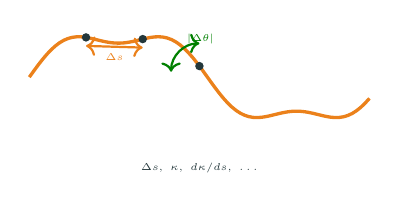
\begin{tikzpicture}[scale=0.72, transform shape]
  \draw[mLightBrown, very thick] plot[domain=0:6, samples=80]
        ({\x},{0.8*sin(deg(\x))+0.2*sin(deg(3*\x))});
  \foreach \px in {1.0,2.0,3.0}{
    \node[circle, fill=mDarkTeal, inner sep=1.5pt] at (\px,{0.8*sin(deg(\px))+0.2*sin(deg(3*\px))}) {};}
  \draw[<->, accent, thick] (1.0,{0.8*sin(deg(1))+0.2*sin(deg(3))-0.15})
      -- (2.0,{0.8*sin(deg(2))+0.2*sin(deg(6))-0.15})
      node[midway, below, font=\tiny\itshape, accent] {$\Delta s$};
  \draw[<->, success, thick] (3.0,{0.8*sin(deg(3))+0.2*sin(deg(9))+0.4})
      arc (90:180:0.5) node[midway, above right, font=\tiny\itshape, success] {$|\Delta\theta|$};
  \node[font=\tiny, mDarkTeal] at (3.0,-1.6) {$\Delta s,\ \kappa,\ d\kappa/ds,\ \ldots$};
\end{tikzpicture}\\[0.3em]
\scriptsize\textit{Các đại lượng nội tại tính trên từng cặp điểm liền kề — không thay đổi khi xoay/tịnh tiến.}
\end{columns}
\end{frame}

% --- Step 2: architecture stack ---
\begin{frame}{Bước 2: Kiến trúc SE2RoadNet (InvariantBlock $\times$6)}
\begin{columns}[c]
\column{0.46\textwidth}
\centering
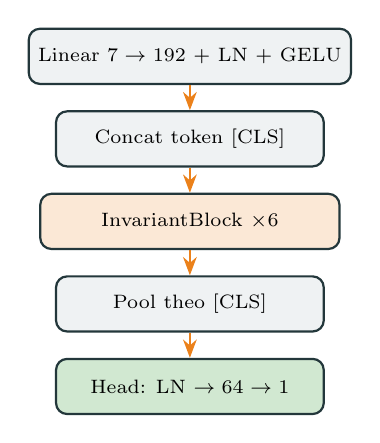
\begin{tikzpicture}[
    box/.style={draw=mDarkTeal, thick, rounded corners, fill=tealtint!40,
                minimum width=3.4cm, minimum height=0.7cm, align=center, font=\scriptsize},
    arr/.style={-Stealth, thick, mLightBrown}
]
  \node[box] (proj) {Linear $7\to192$ + LN + GELU};
  \node[box, below=0.32cm of proj] (cls) {Concat token [CLS]};
  \node[box, below=0.32cm of cls, fill=mLightBrown!18, minimum width=3.8cm] (blk1) {InvariantBlock $\times 6$};
  \node[box, below=0.32cm of blk1] (pool) {Pool theo [CLS]};
  \node[box, below=0.32cm of pool, fill=success!18] (head) {Head: LN $\to 64 \to 1$};
  \draw[arr] (proj) -- (cls);
  \draw[arr] (cls) -- (blk1);
  \draw[arr] (blk1) -- (pool);
  \draw[arr] (pool) -- (head);
\end{tikzpicture}

\column{0.50\textwidth}
\footnotesize
\begin{itemize}\setlength{\itemsep}{4pt}
  \item Mỗi điểm trên đường $\Rightarrow$ một \textbf{token 192 chiều}.
  \item \textbf{Mỗi block} $=$ MHA (8 heads) + FFN (512) + LayerNorm, với \textbf{relative-arclength bias} (Bước 3).
  \item Pool \texttt{[CLS]} $\to$ 1 logit $=$ xác suất FAIL.
\end{itemize}
\vspace{0.3em}
\begin{exampleblock}{Quy mô}
\scriptsize Tổng \textbf{2.11 M} tham số ($\sim$2.5$\times$ RoadFury) — vẫn nhẹ, train 24 phút.
\end{exampleblock}
\end{columns}
\end{frame}

% --- Step 3: relative-Δs attention bias (TikZ, replaces PNG) ---
\begin{frame}{Bước 3: Attention với bias hiệu số $\Delta s$}
\begin{columns}[T]
\column{0.48\textwidth}
\begin{block}{Vấn đề với PE tuyệt đối}
\scriptsize
PE chuẩn (sin/cos của index $i$) khoá mô hình vào \textbf{vị trí tuyệt đối} của token. Xoay/cắt đường khác $\Rightarrow$ index ứng với arclength khác $\Rightarrow$ vỡ bất biến.
\end{block}
\begin{block}{Giải pháp: relative-arclength RFF bias}
\scriptsize
Thêm bias vào ma trận attention, chỉ phụ thuộc \textbf{hiệu số} $\Delta s_{ij}=s_i-s_j$ (bất biến tái tham số hoá):
\[
\mathrm{bias}_{ij}=\mathrm{MLP}\bigl(\sin(\Delta s_{ij}\cdot\omega)\bigr)\in\mathbb{R}^{8}
\]
với $\omega\in\mathbb{R}^{32}$ là tần số Fourier ngẫu nhiên (RFF) cố định.
\end{block}

\column{0.50\textwidth}
\centering
% --- pure-TikZ schematic ---
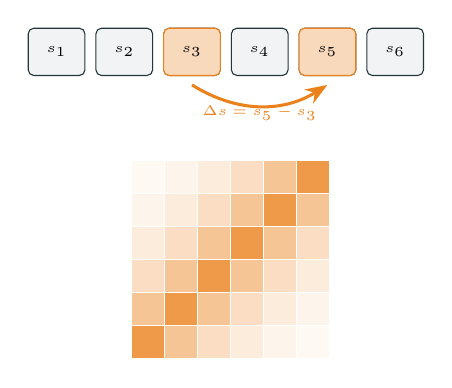
\begin{tikzpicture}[font=\scriptsize,
  tok/.style={draw=mDarkTeal, rounded corners=2pt, fill=tealtint!35,
              minimum width=0.72cm, minimum height=0.6cm, font=\tiny}]
  \foreach \i [count=\c from 0] in {1,2,3,4,5,6}{
    \node[tok] (t\i) at (\c*0.86,3.2) {$s_{\i}$};}
  \node[tok, fill=mLightBrown!30, draw=mLightBrown] at (2*0.86,3.2) {$s_{3}$};
  \node[tok, fill=mLightBrown!30, draw=mLightBrown] at (4*0.86,3.2) {$s_{5}$};
  \draw[-{Stealth}, mLightBrown, line width=1.1pt] (2*0.86,2.78) to[bend right=32] (4*0.86,2.78);
  \node[mLightBrown, font=\tiny] at (3*0.86,2.42) {$\Delta s=s_5-s_3$};
  % mini 6x6 heatmap: intensity decays with |i-j|
  \begin{scope}[shift={(0.95,-0.7)}]
    \foreach \i in {0,...,5}{ \foreach \j in {0,...,5}{
      \pgfmathsetmacro\d{abs(\i-\j)}
      \pgfmathsetmacro\op{80*exp(-0.55*\d)}
      \fill[mLightBrown!\op] (\j*0.42,\i*0.42) rectangle ++(0.42,0.42);
      \draw[white, line width=0.4pt] (\j*0.42,\i*0.42) rectangle ++(0.42,0.42);}}
  \end{scope}
\end{tikzpicture}\\[0.2em]
\scriptsize\textit{Heatmap: attention giảm theo $|\Delta s_{ij}|$ — bias chỉ phụ thuộc hiệu số, không bao giờ $i,j$ riêng lẻ.}
\end{columns}

\takeaway{Chi phí: $\mathcal{O}(B\cdot L^2\cdot 32)$ mỗi block — điểm tốn nhất (24 phút train). Cải tiến tương lai: RoPE-1D trên $s_{\text{norm}}$.}
\end{frame}

% --- Step 4: training (focal loss chart + config) ---
\begin{frame}{Bước 4: Huấn luyện}
\begin{columns}[c]
\column{0.52\textwidth}
\centering
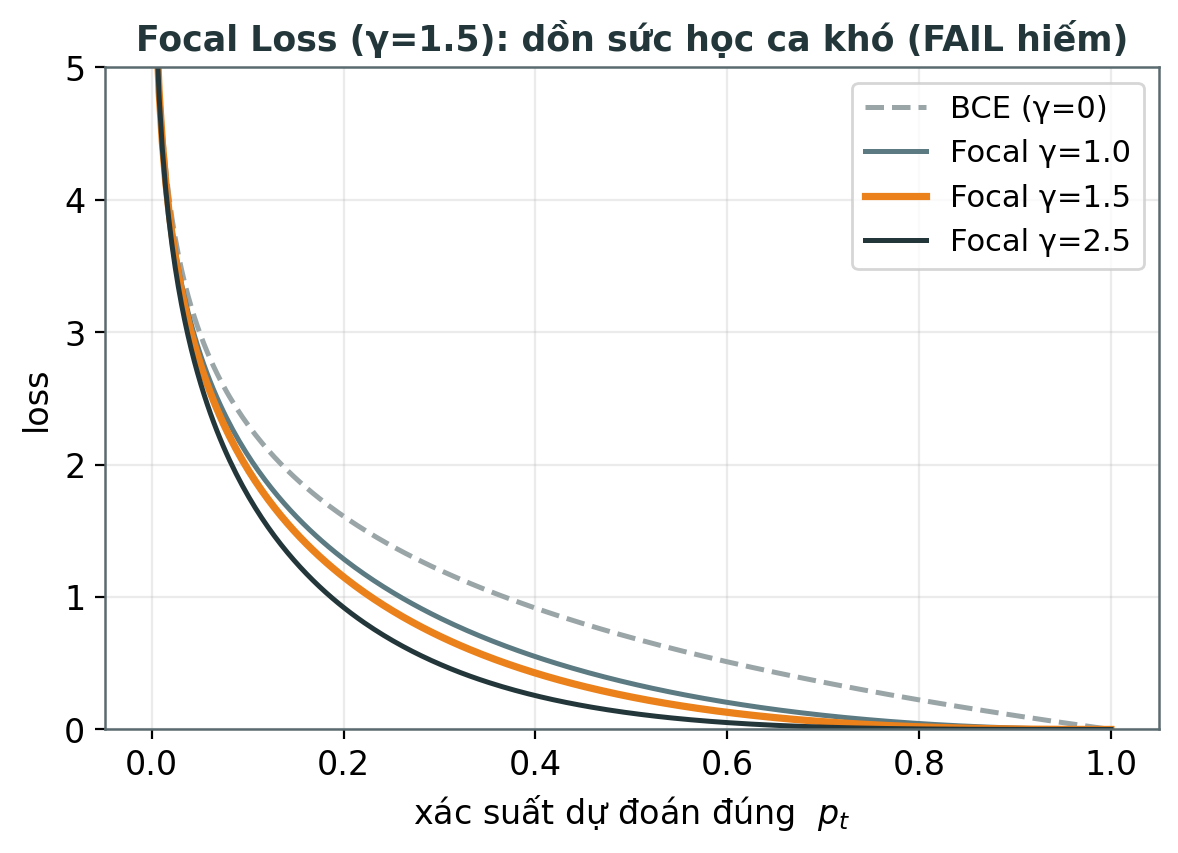
\includegraphics[width=\linewidth]{gen_focal_loss.png}

\column{0.44\textwidth}
\begin{block}{Vì sao Focal Loss?}
\scriptsize
\[
\mathcal{L}=-\alpha(1-\hat p_t)^\gamma\log\hat p_t,\quad \gamma=1.5.
\]
FAIL chỉ $\sim$30--40\%; BCE thuần $\Rightarrow$ model ``đoán PASS hết''. Hệ số $(1-\hat p_t)^\gamma$ \emph{down-weight} ca dễ, \emph{up-weight} ca khó.
\end{block}
\begin{block}{Cấu hình}
\scriptsize
\setlength{\tabcolsep}{3pt}
\begin{tabular}{@{}ll@{}}
Optimizer & AdamW (wd 1e-3) \\
LR        & 5e-4 cosine + warmup 5 \\
Batch / Epochs & 384 / 80 (SWA từ 56) \\
Precision & bf16 \quad Sampler: WeightedRandom \\
Wall-clock & 24.2 phút \quad Params: \textbf{2.11 M} \\
\end{tabular}
\end{block}
\end{columns}
\end{frame}

% ============================================================
\section{Đánh giá thực nghiệm}
% ============================================================

% --- APFD metric ---
\begin{frame}{Chỉ số đánh giá: APFD}
\begin{columns}[c]
\column{0.48\textwidth}
\begin{block}{Average Percentage of Faults Detected}
\small
Với hoán vị $\pi$ trên $n$ test ($m$ là FAIL), $TF_i$ là vị trí fault thứ $i$:
\[
\mathrm{APFD}(\pi)=1-\frac{\sum_{i=1}^{m}TF_i}{n\cdot m}+\frac{1}{2n}.
\]
\textbf{Khoảng}: $[0,1]$, càng cao càng tốt.\\[3pt]
\textbf{Ngẫu nhiên} $\approx 0.5$;\quad \textbf{Lý tưởng} $\approx 1.0$.
\end{block}

\column{0.50\textwidth}
\centering
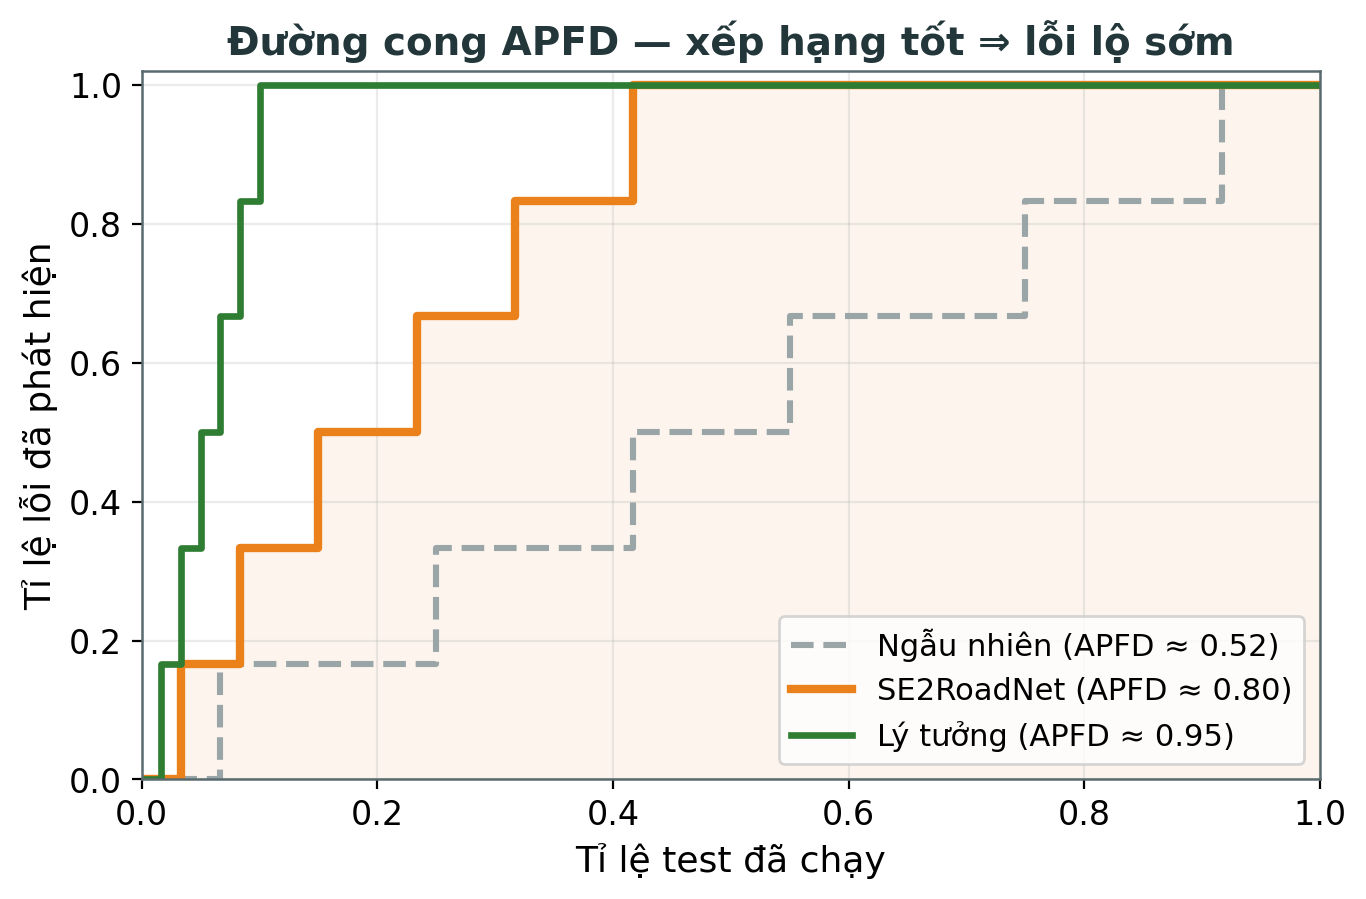
\includegraphics[width=\linewidth]{gen_apfd_curve.png}\\[0.2em]
\scriptsize\textit{Ranking tốt $\Rightarrow$ đường cong tăng dốc đứng từ đầu.}
\end{columns}
\end{frame}

% --- Eval protocol (TikZ, replaces PNG) ---
\begin{frame}{Giao thức đánh giá}
\centering
\begin{tikzpicture}[font=\scriptsize,
  panelbase/.style={rounded corners=6pt, line width=1pt,
                text width=3.6cm, minimum height=3.7cm, align=center, inner sep=7pt, anchor=north},
  panelN/.style={panelbase, draw=navydeep!55, fill=navydeep!6},
  panelO/.style={panelbase, draw=mLightBrown!55, fill=mLightBrown!6},
  panelG/.style={panelbase, draw=success!55, fill=success!6},
  arr/.style={-{Stealth[length=2.5mm]}, line width=1.2pt, mDarkTeal!70},
]
  % Panel 1
  \node[panelN] (p1) at (-4.4,3.0) {%
    \textbf{\color{navydeep}1. Single-pass}\\[4pt]
    \textcolor{navydeep!30}{\rule{\linewidth}{0.5pt}}\\[5pt]
    Xếp hạng 1 lần trên toàn\\ Competition split (956 test)\\[8pt]
    \fcolorbox{navydeep}{navydeep!12}{\footnotesize\bfseries APFD $=0.8047$}};
  % Panel 2
  \node[panelO] (p2) at (0,3.0) {%
    \textbf{\color{mLightBrown!85!black}2. Multi-trial (30 lần)}\\[4pt]
    \textcolor{mLightBrown!30}{\rule{\linewidth}{0.5pt}}\\[5pt]
    Mỗi trial: lấy ngẫu nhiên\\ $287/956$ test $\to$ APFD\\[8pt]
    \fcolorbox{mLightBrown}{mLightBrown!12}{\footnotesize\bfseries $0.8048\pm 0.0118$}\\[4pt]
    {\tiny loại ``may rủi'' do thứ tự cố định}};
  % Panel 3
  \node[panelG] (p3) at (4.4,3.0) {%
    \textbf{\color{success!55!black}3. Rotation probe}\\[4pt]
    \textcolor{success!40!black!30}{\rule{\linewidth}{0.5pt}}\\[5pt]
    Xoay \emph{toàn bộ} split bằng\\ $\{0,30,60,90,180,-45\}^\circ$\\ rồi đánh giá lại\\[6pt]
    \fcolorbox{success!55!black}{success!18}{\footnotesize\bfseries $\Delta=\max-\min$ APFD}};
  \draw[arr] (p1.east) -- (p2.west);
  \draw[arr] (p2.east) -- (p3.west);
\end{tikzpicture}

\takeaway{Ba lớp: single-pass (điểm chính) $\to$ multi-trial (độ ổn định) $\to$ rotation probe (kiểm chứng bất biến).}
\end{frame}

% --- HEADLINE: rotation invariance Δ=0 ---
\begin{frame}{Kết quả headline: Bất biến phép xoay $\Delta=0$}
\begin{columns}[c]
\column{0.52\textwidth}
\centering
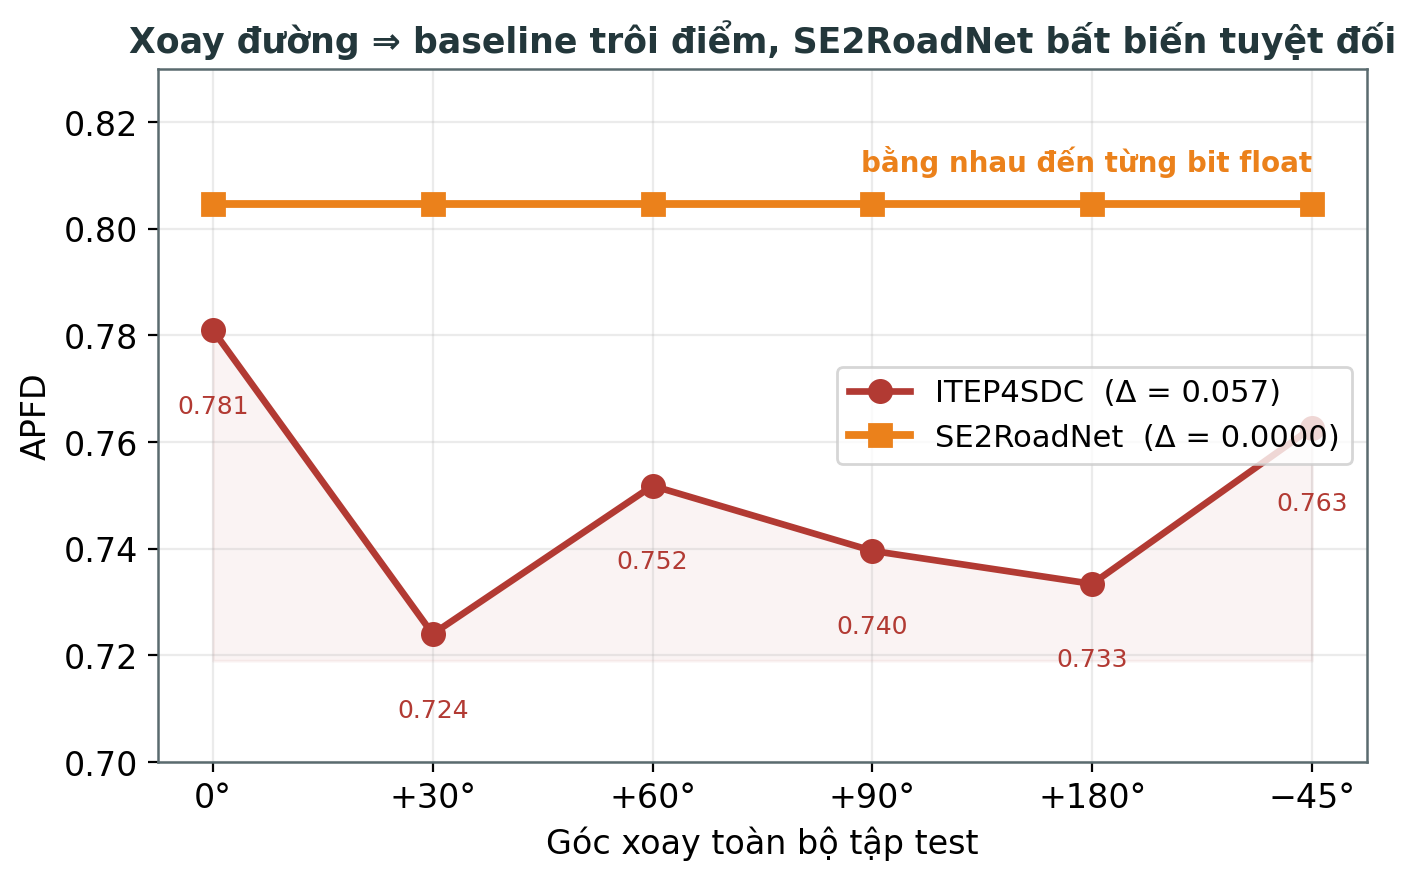
\includegraphics[width=\linewidth]{gen_rotation_drift.png}

\column{0.46\textwidth}
\scriptsize
\setlength{\tabcolsep}{3pt}
\begin{tabular}{l c c c}
\toprule
\textbf{Xoay} & \textbf{ITEP4SDC} & \textbf{SE2RoadNet} \\
\midrule
$0^\circ$    & 0.7810 & \textbf{0.8047} \\
$+30^\circ$  & 0.7240 & \textbf{0.8047} \\
$+60^\circ$  & 0.7518 & \textbf{0.8047} \\
$+90^\circ$  & 0.7396 & \textbf{0.8047} \\
$+180^\circ$ & 0.7334 & \textbf{0.8047} \\
$-45^\circ$  & 0.7627 & \textbf{0.8047} \\
\midrule
$\Delta$ & \alert{0.0570} & \cellcolor{success!25}\textbf{0.0000} \\
\bottomrule
\end{tabular}

\vspace{0.4em}
\begin{exampleblock}{Không phải ``trong sai số''}
\scriptsize
6 góc xoay, APFD bằng nhau \textbf{đến từng bit float} ($=0$, không phải $\sim 10^{-3}$): pipeline 7 kênh trả vector \emph{pixel-identical} sau xoay $\Rightarrow$ logit y nguyên.
\end{exampleblock}
\end{columns}

\vspace{0.2em}
\centering\textcolor{accent}{$\Rightarrow$ \textbf{Lý thuyết được xác minh bằng thực nghiệm}, không cần nói ``xấp xỉ''.}
\end{frame}

% --- Leaderboard ---
\begin{frame}{Bảng xếp hạng: so với 8 baselines}
\begin{columns}[c]
\column{0.56\textwidth}
\centering
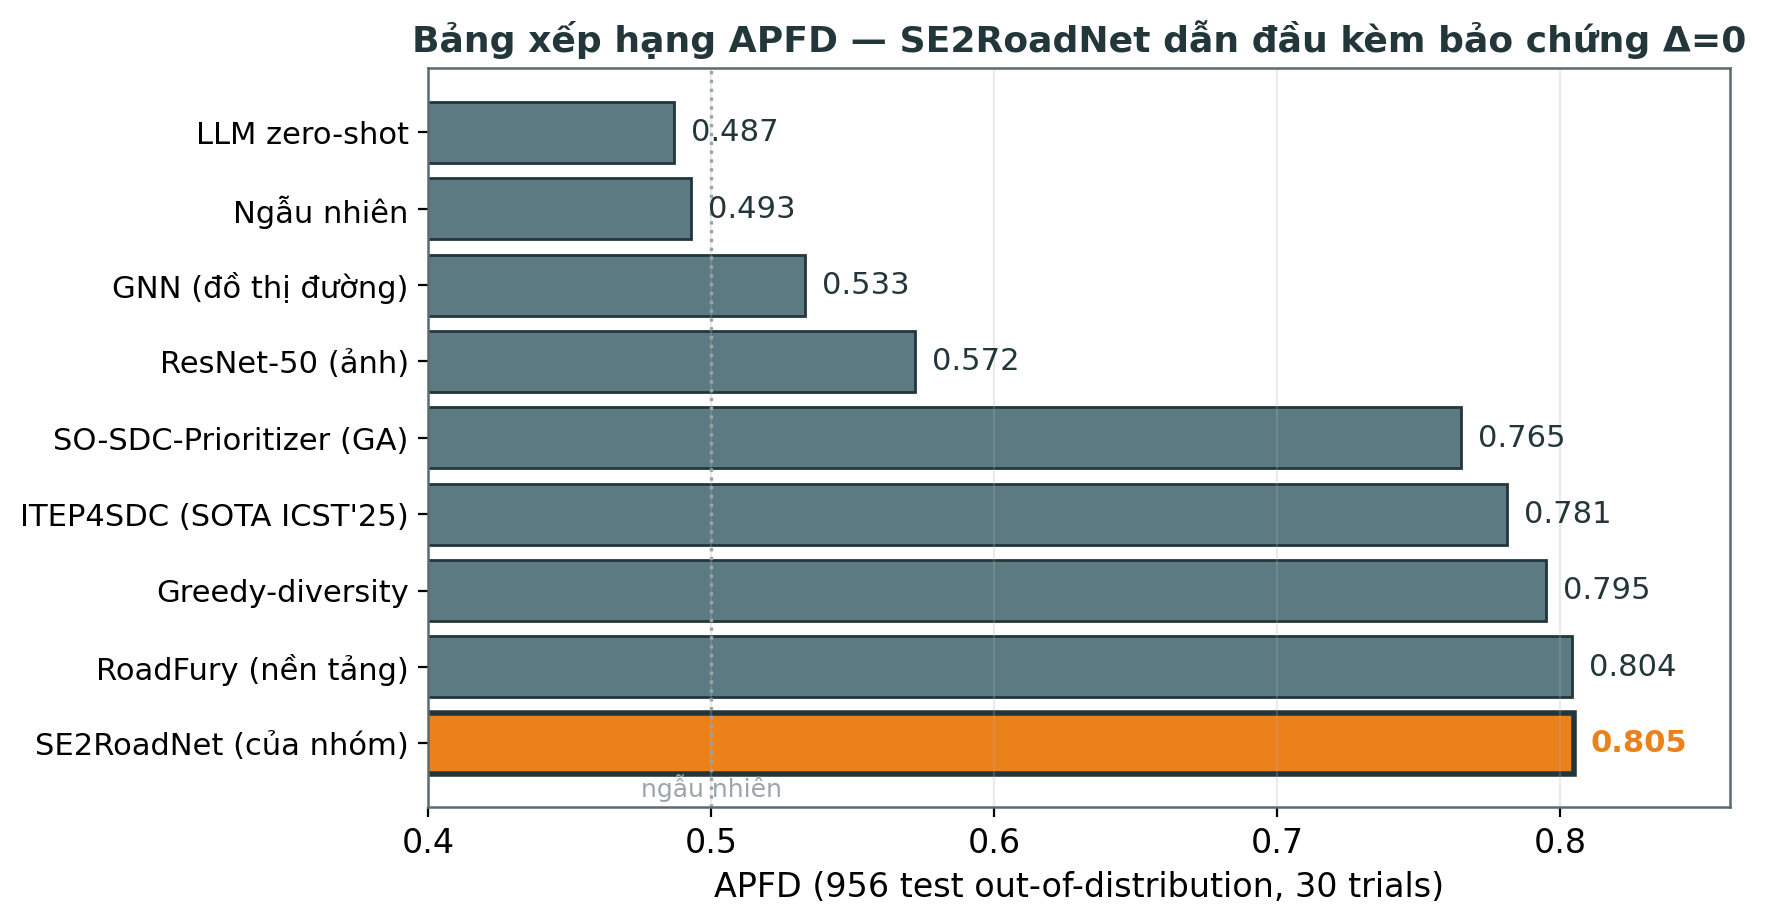
\includegraphics[width=\linewidth]{gen_leaderboard.png}

\column{0.42\textwidth}
\scriptsize
\setlength{\tabcolsep}{4pt}
\begin{tabular}{@{}l c c@{}}
\toprule
\textbf{Method} & \textbf{AUC} & \textbf{APFD} \\
\midrule
RoadFury           & 0.917 & 0.804 \\
\rowcolor{success!15}
\textbf{SE2RoadNet} & \textbf{0.934} & \textbf{0.805} \\
\bottomrule
\end{tabular}

\vspace{0.5em}
\begin{exampleblock}{Đọc bảng}
\scriptsize
SE2RoadNet \textbf{ngang APFD} baseline tốt nhất, nhưng \textbf{tăng AUC} ($+0.017$) và \textbf{thêm bảo chứng} $\Delta=0$ mà không method nào có $\Rightarrow$ cải thiện theo nghĩa \emph{Pareto}.
\end{exampleblock}
\end{columns}

\takeaway{Không đánh đổi: giữ APFD đỉnh, tăng AUC, và là phương pháp duy nhất bất biến SE(2) tuyệt đối.}
\end{frame}

% ============================================================
\section{Hạn chế \& Hướng phát triển}
% ============================================================

% --- Limitations (honest) ---
\begin{frame}{Hạn chế: nhìn thẳng vào điểm yếu}
\begin{columns}[T,onlytextwidth]
\column{0.50\textwidth}
\scriptsize
\textbf{\color{navydeep}Về chỉ số}
\begin{itemize}\setlength{\itemsep}{0.4em}
  \item \textcolor{alert!80!black}{\textbf{AUC và APFD phân kỳ:}} AUC cao hơn không kéo theo APFD cao hơn — phải lập luận cẩn thận metric nào quan trọng khi nào.
  \item \textcolor{alert!80!black}{\textbf{Listwise loss chưa tăng APFD trung bình:}} chỉ giảm $\sigma$ $\Rightarrow$ đóng góp ``ổn định'', không phải headline.
  \item \textcolor{alert!80!black}{\textbf{Trần APFD ở bench FAIL cao:}} ví dụ 95\% FAIL $\Rightarrow$ APFD $\approx 0.52$ là \emph{ceiling}, không phải thất bại.
\end{itemize}

\column{0.46\textwidth}
\scriptsize
\textbf{\color{navydeep}Về phương pháp}
\begin{itemize}\setlength{\itemsep}{0.4em}
  \item \textcolor{alert!80!black}{\textbf{Conformal an toàn còn dở:}} v1 valid-nhưng-vô nghĩa, v2 informative-nhưng-invalid; cần v3 mới ship.
  \item \textcolor{alert!80!black}{\textbf{Dịch phân phối chưa đóng:}} IRM / TENT chưa thu hẹp gap SensoDat$\to$Competition (negative đã biết).
  \item \textcolor{alert!80!black}{\textbf{Bất biến lấy mẫu là xấp xỉ:}} resolution probe $\Delta\!\approx\!0.0012$ (rất nhỏ) — chưa \emph{exact} như phép xoay.
\end{itemize}
\end{columns}

\takeaway{Bất biến xoay là \emph{exact}; các đảm bảo khác (resolution, conformal) vẫn đang hoàn thiện — báo cáo trung thực thay vì giấu.}
\end{frame}

% --- Future work ---
\begin{frame}{Hướng phát triển}
\centering
\begin{tikzpicture}[font=\scriptsize,
  fwcard/.style={draw=mLightBrown!45, fill=mLightBrown!5, rounded corners=6pt, line width=1pt,
                 text width=5.3cm, minimum height=1.95cm, align=left, inner sep=10pt, anchor=center},
  wm/.style={font=\Huge\bfseries, text=mLightBrown!25},
]
  \def\xl{-3.2}\def\xr{3.2}\def\yt{1.55}\def\yb{-0.75}
  \node[fwcard] (c1) at (\xl,\yt) {\textbf{\normalsize\color{navydeep}Tổng quát hoá đa benchmark}\\[3pt]{\tiny Một công thức, 8+ benchmark công khai (OOB, SDC-Scissor, sdc-travel\dots) — APFD không tinh chỉnh theo từng bench.}};
  \node[fwcard] (c2) at (\xr,\yt) {\textbf{\normalsize\color{navydeep}An toàn có bảo chứng (Conformal v3)}\\[3pt]{\tiny Chặn dưới prefix-APFD vừa \emph{valid} vừa \emph{non-vacuous}; audit tỉ lệ vi phạm độ cong.}};
  \node[fwcard] (c3) at (\xl,\yb) {\textbf{\normalsize\color{navydeep}Bất biến lấy mẫu \emph{exact}}\\[3pt]{\tiny RoPE-1D trên $s_{\text{norm}}$ thay RFF bias $\Rightarrow$ rẻ hơn và tiến tới resolution-$\Delta=0$.}};
  \node[fwcard] (c4) at (\xr,\yb) {\textbf{\normalsize\color{navydeep}SSL vật lý (physics-informed)}\\[3pt]{\tiny Pretext task gắn với độ cong/jerk để học biểu diễn nền — thay SSL hình học ngây thơ (chuyển kém).}};
  \foreach \c/\n in {c1/1,c2/2,c3/3,c4/4}{
    \node[wm, anchor=north east] at ([xshift=-5pt,yshift=-3pt]\c.north east) {\n};}
\end{tikzpicture}

\vspace{0.4em}
{\centering\footnotesize\color{mDarkTeal}$\Rightarrow$ Mục tiêu: từ một baseline bất biến cho SDC $\to$ \textbf{công thức chung} bất biến \& audit-readable cho mọi benchmark.\par}
\end{frame}

% --- References ---
\begin{frame}{Tài liệu tham khảo}
\footnotesize
\begin{enumerate}\setlength{\itemsep}{0.32em}
  \item C. Birchler, C. Rohrbach, T. Kehrer, S. Panichella. \textit{SensoDat: Simulation-based Sensor Dataset of Self-driving Cars}. MSR 2024. {\scriptsize\color{gray}(nguồn dataset)}
  \item C. Birchler, S. Khatiri, B. Bosshard, A. Gambi, S. Panichella. \textit{Single and Multi-objective Test Cases Prioritization for Self-driving Cars in Virtual Environments}. ACM TOSEM, 2023. {\scriptsize\color{gray}(SO-SDC-Prioritizer)}
  \item \textit{ICST/SBFT Tool Competition -- Self-Driving Car Testing (Cyber-Physical Systems)}. 2023--2025. {\scriptsize\color{gray}(ITEP4SDC, giao thức APFD competition)}
  \item G. Rothermel, R. Untch, C. Chu, M. Harrold. \textit{Prioritizing Test Cases for Regression Testing}. IEEE TSE, 2001. {\scriptsize\color{gray}(định nghĩa APFD)}
  \item A. Vaswani et al. \textit{Attention Is All You Need}. NeurIPS 2017.
  \item T.-Y. Lin, P. Goyal, R. Girshick, K. He, P. Dollár. \textit{Focal Loss for Dense Object Detection}. ICCV 2017.
  \item P. Izmailov et al. \textit{Averaging Weights Leads to Wider Optima and Better Generalization} (\textbf{SWA}). UAI 2018.
  \item T. Cohen, M. Welling. \textit{Group Equivariant Convolutional Networks}. ICML 2016. {\scriptsize\color{gray}(nền tảng bất biến nhóm)}
  \item A. Rahimi, B. Recht. \textit{Random Features for Large-Scale Kernel Machines} (\textbf{RFF}). NeurIPS 2007.
  \item A. Angelopoulos, S. Bates. \textit{A Gentle Introduction to Conformal Prediction}. 2021. {\scriptsize\color{gray}(hướng an toàn)}
\end{enumerate}
\end{frame}

% --- Thank you ---
{
\setbeamertemplate{footline}{}
\begin{frame}{Cảm ơn!}
\vspace{1.4em}
\centering
\Large\textbf{\color{mDarkTeal}Cảm ơn thầy đã lắng nghe!}\\[1em]
\large\textit{Q\&A — Questions \& Discussion}

\vspace{1.6em}
\scriptsize
\begin{columns}[c]
\column{0.18\textwidth}
\centering

\includegraphics[height=1.4cm]{hcmus.png}

\column{0.64\textwidth}
\centering
\textcolor{navydeep}{\textbf{Test Prioritization for Self-Driving Cars}}\\[0.2em]
SE2RoadNet — bất biến SE(2) bằng kiến trúc\\[0.4em]
Trần Chí Nguyên $\cdot$ Huỳnh Trung Kiệt $\cdot$ Đào Sỹ Duy Minh\\[0.2em]
University of Science, VNU-HCM $\cdot$ ICST 2026

\column{0.18\textwidth}
\centering

\includegraphics[height=1.1cm]{icst_logo.jpg}
\end{columns}
\end{frame}
}

% ============================================================
% BACKUP SLIDES (Q&A)
% ============================================================
\appendix

\begin{frame}{Backup: APFD — ví dụ tính tay}
\footnotesize
Giả sử $n=5$ test, $m=2$ FAIL. Hai cách xếp hạng:
\vspace{0.4em}
\begin{columns}[T]
\column{0.5\textwidth}
\centering
\textbf{Xếp tốt} (FAIL ở vị trí 1, 2)
\[
\mathrm{APFD}=1-\frac{1+2}{5\cdot 2}+\frac{1}{10}=\mathbf{0.80}
\]
\column{0.5\textwidth}
\centering
\textbf{Xếp kém} (FAIL ở vị trí 4, 5)
\[
\mathrm{APFD}=1-\frac{4+5}{5\cdot 2}+\frac{1}{10}=\mathbf{0.20}
\]
\end{columns}
\vspace{0.6em}
\takeaway{Cùng một tập lỗi — chỉ khác \emph{thứ tự} — APFD chênh nhau 4 lần. Đó là toàn bộ giá trị của test prioritization.}
\end{frame}

\begin{frame}{Backup: Multi-trial protocol (vì sao 30 lần?)}
\footnotesize
\begin{itemize}\setlength{\itemsep}{0.5em}
  \item APFD single-pass nhạy với \emph{thứ tự cố định} của tập test $\Rightarrow$ một con số dễ ``may rủi''.
  \item Mỗi trial: lấy ngẫu nhiên $\max(50,\ 0.3\cdot|test|)=287/956$ test, tính APFD độc lập.
  \item Báo cáo $\overline{\mathrm{APFD}}\pm\sigma$ qua \textbf{30 trials}, seed $=42$.
  \item $\sigma$ thường là con số xuất bản quan trọng hơn mean (đo độ ổn định của ranking).
\end{itemize}
\centering
\fcolorbox{mLightBrown}{mLightBrown!10}{\parbox{0.8\linewidth}{\centering
  SE2RoadNet: $0.8048\pm 0.0118$ \quad (mean $\pm\ \sigma$, 30 trials)}}
\end{frame}

\begin{frame}{Backup: AUC vs APFD — vì sao tách bạch?}
\footnotesize
\begin{columns}[T]
\column{0.5\textwidth}
\textbf{\color{navydeep}AUC} đo \emph{khả năng phân loại} PASS/FAIL trên \emph{từng cặp} — không quan tâm thứ hạng tuyệt đối.
\column{0.5\textwidth}
\textbf{\color{mLightBrown}APFD} đo \emph{tốc độ lộ lỗi theo thứ tự chạy} — chính là cái competition tối ưu.
\end{columns}
\vspace{0.5em}
\begin{itemize}\setlength{\itemsep}{0.35em}
  \item Trong gần như mọi thí nghiệm của nhóm, AUC và APFD \textbf{phân kỳ}: tăng AUC không đảm bảo tăng APFD.
  \item SE2RoadNet tăng AUC ($0.917\to 0.934$) trong khi APFD giữ đỉnh ($\approx 0.805$).
  \item $\Rightarrow$ Khi báo cáo phải nói rõ \emph{metric nào} đang được tối ưu cho tình huống nào.
\end{itemize}
\takeaway{Không gộp AUC và APFD thành ``một điểm tốt hơn'' — chúng đo hai thứ khác nhau.}
\end{frame}

\begin{frame}{Backup: Resolution probe (bất biến lấy mẫu)}
\footnotesize
\begin{itemize}\setlength{\itemsep}{0.5em}
  \item Lấy cùng một con đường, resample ở $N\in\{64,\dots,197\}$ điểm rồi đánh giá lại.
  \item Đo $\Delta=\max-\min$ APFD qua các mức $N$.
  \item Kết quả: $\Delta\approx \mathbf{0.0012}$ — \emph{rất nhỏ} nhưng \textbf{chưa exact} như phép xoay ($\Delta=0$).
  \item Lý do: bias RFF theo $\Delta s$ là gần-bất-biến tái tham số hoá, không tuyệt đối $\Rightarrow$ hướng RoPE-1D.
\end{itemize}
\takeaway{Phép xoay: $\Delta=0$ exact (bằng kiến trúc). Lấy mẫu: $\Delta\approx 0.0012$ (gần như, đang tiến tới exact).}
\end{frame}

\begin{frame}{Backup: Chi phí ở quy mô lớn}
\footnotesize
\begin{itemize}\setlength{\itemsep}{0.5em}
  \item Inference: \textbf{1 forward pass}/đường, batch $(n,7,197)$ $\Rightarrow$ chấm cả tập trong vài giây GPU.
  \item Chi phí thật nằm ở \emph{mô phỏng vật lý} của các test được chọn — không phải ở scorer.
  \item Ranking tốt cắt 50--80\% số kịch bản cần chạy mô phỏng $\Rightarrow$ tiết kiệm \textbf{nhiều giờ CPU}.
  \item Train một lần: 24.2 phút (Kaggle), 2.11 M tham số $\Rightarrow$ tái lập rẻ.
\end{itemize}
\takeaway{``The best simulation is the one you never run.'' — scorer rẻ, ngân sách dồn cho các test có khả năng lộ lỗi cao nhất.}
\end{frame}

\end{document}
